
% Default to the notebook output style

    


% Inherit from the specified cell style.




    
\documentclass[11pt]{article}

    
    
    \usepackage[T1]{fontenc}
    % Nicer default font (+ math font) than Computer Modern for most use cases
    \usepackage{mathpazo}

    % Basic figure setup, for now with no caption control since it's done
    % automatically by Pandoc (which extracts ![](path) syntax from Markdown).
    \usepackage{graphicx}
    % We will generate all images so they have a width \maxwidth. This means
    % that they will get their normal width if they fit onto the page, but
    % are scaled down if they would overflow the margins.
    \makeatletter
    \def\maxwidth{\ifdim\Gin@nat@width>\linewidth\linewidth
    \else\Gin@nat@width\fi}
    \makeatother
    \let\Oldincludegraphics\includegraphics
    % Set max figure width to be 80% of text width, for now hardcoded.
    \renewcommand{\includegraphics}[1]{\Oldincludegraphics[width=.8\maxwidth]{#1}}
    % Ensure that by default, figures have no caption (until we provide a
    % proper Figure object with a Caption API and a way to capture that
    % in the conversion process - todo).
    \usepackage{caption}
    \DeclareCaptionLabelFormat{nolabel}{}
    \captionsetup{labelformat=nolabel}

    \usepackage{adjustbox} % Used to constrain images to a maximum size 
    \usepackage{xcolor} % Allow colors to be defined
    \usepackage{enumerate} % Needed for markdown enumerations to work
    \usepackage{geometry} % Used to adjust the document margins
    \usepackage{amsmath} % Equations
    \usepackage{amssymb} % Equations
    \usepackage{textcomp} % defines textquotesingle
    % Hack from http://tex.stackexchange.com/a/47451/13684:
    \AtBeginDocument{%
        \def\PYZsq{\textquotesingle}% Upright quotes in Pygmentized code
    }
    \usepackage{upquote} % Upright quotes for verbatim code
    \usepackage{eurosym} % defines \euro
    \usepackage[mathletters]{ucs} % Extended unicode (utf-8) support
    \usepackage[utf8x]{inputenc} % Allow utf-8 characters in the tex document
    \usepackage{fancyvrb} % verbatim replacement that allows latex
    \usepackage{grffile} % extends the file name processing of package graphics 
                         % to support a larger range 
    % The hyperref package gives us a pdf with properly built
    % internal navigation ('pdf bookmarks' for the table of contents,
    % internal cross-reference links, web links for URLs, etc.)
    \usepackage{hyperref}
    \usepackage{longtable} % longtable support required by pandoc >1.10
    \usepackage{booktabs}  % table support for pandoc > 1.12.2
    \usepackage[inline]{enumitem} % IRkernel/repr support (it uses the enumerate* environment)
    \usepackage[normalem]{ulem} % ulem is needed to support strikethroughs (\sout)
                                % normalem makes italics be italics, not underlines
    

    
    
    % Colors for the hyperref package
    \definecolor{urlcolor}{rgb}{0,.145,.698}
    \definecolor{linkcolor}{rgb}{.71,0.21,0.01}
    \definecolor{citecolor}{rgb}{.12,.54,.11}

    % ANSI colors
    \definecolor{ansi-black}{HTML}{3E424D}
    \definecolor{ansi-black-intense}{HTML}{282C36}
    \definecolor{ansi-red}{HTML}{E75C58}
    \definecolor{ansi-red-intense}{HTML}{B22B31}
    \definecolor{ansi-green}{HTML}{00A250}
    \definecolor{ansi-green-intense}{HTML}{007427}
    \definecolor{ansi-yellow}{HTML}{DDB62B}
    \definecolor{ansi-yellow-intense}{HTML}{B27D12}
    \definecolor{ansi-blue}{HTML}{208FFB}
    \definecolor{ansi-blue-intense}{HTML}{0065CA}
    \definecolor{ansi-magenta}{HTML}{D160C4}
    \definecolor{ansi-magenta-intense}{HTML}{A03196}
    \definecolor{ansi-cyan}{HTML}{60C6C8}
    \definecolor{ansi-cyan-intense}{HTML}{258F8F}
    \definecolor{ansi-white}{HTML}{C5C1B4}
    \definecolor{ansi-white-intense}{HTML}{A1A6B2}

    % commands and environments needed by pandoc snippets
    % extracted from the output of `pandoc -s`
    \providecommand{\tightlist}{%
      \setlength{\itemsep}{0pt}\setlength{\parskip}{0pt}}
    \DefineVerbatimEnvironment{Highlighting}{Verbatim}{commandchars=\\\{\}}
    % Add ',fontsize=\small' for more characters per line
    \newenvironment{Shaded}{}{}
    \newcommand{\KeywordTok}[1]{\textcolor[rgb]{0.00,0.44,0.13}{\textbf{{#1}}}}
    \newcommand{\DataTypeTok}[1]{\textcolor[rgb]{0.56,0.13,0.00}{{#1}}}
    \newcommand{\DecValTok}[1]{\textcolor[rgb]{0.25,0.63,0.44}{{#1}}}
    \newcommand{\BaseNTok}[1]{\textcolor[rgb]{0.25,0.63,0.44}{{#1}}}
    \newcommand{\FloatTok}[1]{\textcolor[rgb]{0.25,0.63,0.44}{{#1}}}
    \newcommand{\CharTok}[1]{\textcolor[rgb]{0.25,0.44,0.63}{{#1}}}
    \newcommand{\StringTok}[1]{\textcolor[rgb]{0.25,0.44,0.63}{{#1}}}
    \newcommand{\CommentTok}[1]{\textcolor[rgb]{0.38,0.63,0.69}{\textit{{#1}}}}
    \newcommand{\OtherTok}[1]{\textcolor[rgb]{0.00,0.44,0.13}{{#1}}}
    \newcommand{\AlertTok}[1]{\textcolor[rgb]{1.00,0.00,0.00}{\textbf{{#1}}}}
    \newcommand{\FunctionTok}[1]{\textcolor[rgb]{0.02,0.16,0.49}{{#1}}}
    \newcommand{\RegionMarkerTok}[1]{{#1}}
    \newcommand{\ErrorTok}[1]{\textcolor[rgb]{1.00,0.00,0.00}{\textbf{{#1}}}}
    \newcommand{\NormalTok}[1]{{#1}}
    
    % Additional commands for more recent versions of Pandoc
    \newcommand{\ConstantTok}[1]{\textcolor[rgb]{0.53,0.00,0.00}{{#1}}}
    \newcommand{\SpecialCharTok}[1]{\textcolor[rgb]{0.25,0.44,0.63}{{#1}}}
    \newcommand{\VerbatimStringTok}[1]{\textcolor[rgb]{0.25,0.44,0.63}{{#1}}}
    \newcommand{\SpecialStringTok}[1]{\textcolor[rgb]{0.73,0.40,0.53}{{#1}}}
    \newcommand{\ImportTok}[1]{{#1}}
    \newcommand{\DocumentationTok}[1]{\textcolor[rgb]{0.73,0.13,0.13}{\textit{{#1}}}}
    \newcommand{\AnnotationTok}[1]{\textcolor[rgb]{0.38,0.63,0.69}{\textbf{\textit{{#1}}}}}
    \newcommand{\CommentVarTok}[1]{\textcolor[rgb]{0.38,0.63,0.69}{\textbf{\textit{{#1}}}}}
    \newcommand{\VariableTok}[1]{\textcolor[rgb]{0.10,0.09,0.49}{{#1}}}
    \newcommand{\ControlFlowTok}[1]{\textcolor[rgb]{0.00,0.44,0.13}{\textbf{{#1}}}}
    \newcommand{\OperatorTok}[1]{\textcolor[rgb]{0.40,0.40,0.40}{{#1}}}
    \newcommand{\BuiltInTok}[1]{{#1}}
    \newcommand{\ExtensionTok}[1]{{#1}}
    \newcommand{\PreprocessorTok}[1]{\textcolor[rgb]{0.74,0.48,0.00}{{#1}}}
    \newcommand{\AttributeTok}[1]{\textcolor[rgb]{0.49,0.56,0.16}{{#1}}}
    \newcommand{\InformationTok}[1]{\textcolor[rgb]{0.38,0.63,0.69}{\textbf{\textit{{#1}}}}}
    \newcommand{\WarningTok}[1]{\textcolor[rgb]{0.38,0.63,0.69}{\textbf{\textit{{#1}}}}}
    
    
    % Define a nice break command that doesn't care if a line doesn't already
    % exist.
    \def\br{\hspace*{\fill} \\* }
    % Math Jax compatability definitions
    \def\gt{>}
    \def\lt{<}
    % Document parameters
    \title{Shor's Algorithm}
    
    
    

    % Pygments definitions
    
\makeatletter
\def\PY@reset{\let\PY@it=\relax \let\PY@bf=\relax%
    \let\PY@ul=\relax \let\PY@tc=\relax%
    \let\PY@bc=\relax \let\PY@ff=\relax}
\def\PY@tok#1{\csname PY@tok@#1\endcsname}
\def\PY@toks#1+{\ifx\relax#1\empty\else%
    \PY@tok{#1}\expandafter\PY@toks\fi}
\def\PY@do#1{\PY@bc{\PY@tc{\PY@ul{%
    \PY@it{\PY@bf{\PY@ff{#1}}}}}}}
\def\PY#1#2{\PY@reset\PY@toks#1+\relax+\PY@do{#2}}

\expandafter\def\csname PY@tok@w\endcsname{\def\PY@tc##1{\textcolor[rgb]{0.73,0.73,0.73}{##1}}}
\expandafter\def\csname PY@tok@c\endcsname{\let\PY@it=\textit\def\PY@tc##1{\textcolor[rgb]{0.25,0.50,0.50}{##1}}}
\expandafter\def\csname PY@tok@cp\endcsname{\def\PY@tc##1{\textcolor[rgb]{0.74,0.48,0.00}{##1}}}
\expandafter\def\csname PY@tok@k\endcsname{\let\PY@bf=\textbf\def\PY@tc##1{\textcolor[rgb]{0.00,0.50,0.00}{##1}}}
\expandafter\def\csname PY@tok@kp\endcsname{\def\PY@tc##1{\textcolor[rgb]{0.00,0.50,0.00}{##1}}}
\expandafter\def\csname PY@tok@kt\endcsname{\def\PY@tc##1{\textcolor[rgb]{0.69,0.00,0.25}{##1}}}
\expandafter\def\csname PY@tok@o\endcsname{\def\PY@tc##1{\textcolor[rgb]{0.40,0.40,0.40}{##1}}}
\expandafter\def\csname PY@tok@ow\endcsname{\let\PY@bf=\textbf\def\PY@tc##1{\textcolor[rgb]{0.67,0.13,1.00}{##1}}}
\expandafter\def\csname PY@tok@nb\endcsname{\def\PY@tc##1{\textcolor[rgb]{0.00,0.50,0.00}{##1}}}
\expandafter\def\csname PY@tok@nf\endcsname{\def\PY@tc##1{\textcolor[rgb]{0.00,0.00,1.00}{##1}}}
\expandafter\def\csname PY@tok@nc\endcsname{\let\PY@bf=\textbf\def\PY@tc##1{\textcolor[rgb]{0.00,0.00,1.00}{##1}}}
\expandafter\def\csname PY@tok@nn\endcsname{\let\PY@bf=\textbf\def\PY@tc##1{\textcolor[rgb]{0.00,0.00,1.00}{##1}}}
\expandafter\def\csname PY@tok@ne\endcsname{\let\PY@bf=\textbf\def\PY@tc##1{\textcolor[rgb]{0.82,0.25,0.23}{##1}}}
\expandafter\def\csname PY@tok@nv\endcsname{\def\PY@tc##1{\textcolor[rgb]{0.10,0.09,0.49}{##1}}}
\expandafter\def\csname PY@tok@no\endcsname{\def\PY@tc##1{\textcolor[rgb]{0.53,0.00,0.00}{##1}}}
\expandafter\def\csname PY@tok@nl\endcsname{\def\PY@tc##1{\textcolor[rgb]{0.63,0.63,0.00}{##1}}}
\expandafter\def\csname PY@tok@ni\endcsname{\let\PY@bf=\textbf\def\PY@tc##1{\textcolor[rgb]{0.60,0.60,0.60}{##1}}}
\expandafter\def\csname PY@tok@na\endcsname{\def\PY@tc##1{\textcolor[rgb]{0.49,0.56,0.16}{##1}}}
\expandafter\def\csname PY@tok@nt\endcsname{\let\PY@bf=\textbf\def\PY@tc##1{\textcolor[rgb]{0.00,0.50,0.00}{##1}}}
\expandafter\def\csname PY@tok@nd\endcsname{\def\PY@tc##1{\textcolor[rgb]{0.67,0.13,1.00}{##1}}}
\expandafter\def\csname PY@tok@s\endcsname{\def\PY@tc##1{\textcolor[rgb]{0.73,0.13,0.13}{##1}}}
\expandafter\def\csname PY@tok@sd\endcsname{\let\PY@it=\textit\def\PY@tc##1{\textcolor[rgb]{0.73,0.13,0.13}{##1}}}
\expandafter\def\csname PY@tok@si\endcsname{\let\PY@bf=\textbf\def\PY@tc##1{\textcolor[rgb]{0.73,0.40,0.53}{##1}}}
\expandafter\def\csname PY@tok@se\endcsname{\let\PY@bf=\textbf\def\PY@tc##1{\textcolor[rgb]{0.73,0.40,0.13}{##1}}}
\expandafter\def\csname PY@tok@sr\endcsname{\def\PY@tc##1{\textcolor[rgb]{0.73,0.40,0.53}{##1}}}
\expandafter\def\csname PY@tok@ss\endcsname{\def\PY@tc##1{\textcolor[rgb]{0.10,0.09,0.49}{##1}}}
\expandafter\def\csname PY@tok@sx\endcsname{\def\PY@tc##1{\textcolor[rgb]{0.00,0.50,0.00}{##1}}}
\expandafter\def\csname PY@tok@m\endcsname{\def\PY@tc##1{\textcolor[rgb]{0.40,0.40,0.40}{##1}}}
\expandafter\def\csname PY@tok@gh\endcsname{\let\PY@bf=\textbf\def\PY@tc##1{\textcolor[rgb]{0.00,0.00,0.50}{##1}}}
\expandafter\def\csname PY@tok@gu\endcsname{\let\PY@bf=\textbf\def\PY@tc##1{\textcolor[rgb]{0.50,0.00,0.50}{##1}}}
\expandafter\def\csname PY@tok@gd\endcsname{\def\PY@tc##1{\textcolor[rgb]{0.63,0.00,0.00}{##1}}}
\expandafter\def\csname PY@tok@gi\endcsname{\def\PY@tc##1{\textcolor[rgb]{0.00,0.63,0.00}{##1}}}
\expandafter\def\csname PY@tok@gr\endcsname{\def\PY@tc##1{\textcolor[rgb]{1.00,0.00,0.00}{##1}}}
\expandafter\def\csname PY@tok@ge\endcsname{\let\PY@it=\textit}
\expandafter\def\csname PY@tok@gs\endcsname{\let\PY@bf=\textbf}
\expandafter\def\csname PY@tok@gp\endcsname{\let\PY@bf=\textbf\def\PY@tc##1{\textcolor[rgb]{0.00,0.00,0.50}{##1}}}
\expandafter\def\csname PY@tok@go\endcsname{\def\PY@tc##1{\textcolor[rgb]{0.53,0.53,0.53}{##1}}}
\expandafter\def\csname PY@tok@gt\endcsname{\def\PY@tc##1{\textcolor[rgb]{0.00,0.27,0.87}{##1}}}
\expandafter\def\csname PY@tok@err\endcsname{\def\PY@bc##1{\setlength{\fboxsep}{0pt}\fcolorbox[rgb]{1.00,0.00,0.00}{1,1,1}{\strut ##1}}}
\expandafter\def\csname PY@tok@kc\endcsname{\let\PY@bf=\textbf\def\PY@tc##1{\textcolor[rgb]{0.00,0.50,0.00}{##1}}}
\expandafter\def\csname PY@tok@kd\endcsname{\let\PY@bf=\textbf\def\PY@tc##1{\textcolor[rgb]{0.00,0.50,0.00}{##1}}}
\expandafter\def\csname PY@tok@kn\endcsname{\let\PY@bf=\textbf\def\PY@tc##1{\textcolor[rgb]{0.00,0.50,0.00}{##1}}}
\expandafter\def\csname PY@tok@kr\endcsname{\let\PY@bf=\textbf\def\PY@tc##1{\textcolor[rgb]{0.00,0.50,0.00}{##1}}}
\expandafter\def\csname PY@tok@bp\endcsname{\def\PY@tc##1{\textcolor[rgb]{0.00,0.50,0.00}{##1}}}
\expandafter\def\csname PY@tok@fm\endcsname{\def\PY@tc##1{\textcolor[rgb]{0.00,0.00,1.00}{##1}}}
\expandafter\def\csname PY@tok@vc\endcsname{\def\PY@tc##1{\textcolor[rgb]{0.10,0.09,0.49}{##1}}}
\expandafter\def\csname PY@tok@vg\endcsname{\def\PY@tc##1{\textcolor[rgb]{0.10,0.09,0.49}{##1}}}
\expandafter\def\csname PY@tok@vi\endcsname{\def\PY@tc##1{\textcolor[rgb]{0.10,0.09,0.49}{##1}}}
\expandafter\def\csname PY@tok@vm\endcsname{\def\PY@tc##1{\textcolor[rgb]{0.10,0.09,0.49}{##1}}}
\expandafter\def\csname PY@tok@sa\endcsname{\def\PY@tc##1{\textcolor[rgb]{0.73,0.13,0.13}{##1}}}
\expandafter\def\csname PY@tok@sb\endcsname{\def\PY@tc##1{\textcolor[rgb]{0.73,0.13,0.13}{##1}}}
\expandafter\def\csname PY@tok@sc\endcsname{\def\PY@tc##1{\textcolor[rgb]{0.73,0.13,0.13}{##1}}}
\expandafter\def\csname PY@tok@dl\endcsname{\def\PY@tc##1{\textcolor[rgb]{0.73,0.13,0.13}{##1}}}
\expandafter\def\csname PY@tok@s2\endcsname{\def\PY@tc##1{\textcolor[rgb]{0.73,0.13,0.13}{##1}}}
\expandafter\def\csname PY@tok@sh\endcsname{\def\PY@tc##1{\textcolor[rgb]{0.73,0.13,0.13}{##1}}}
\expandafter\def\csname PY@tok@s1\endcsname{\def\PY@tc##1{\textcolor[rgb]{0.73,0.13,0.13}{##1}}}
\expandafter\def\csname PY@tok@mb\endcsname{\def\PY@tc##1{\textcolor[rgb]{0.40,0.40,0.40}{##1}}}
\expandafter\def\csname PY@tok@mf\endcsname{\def\PY@tc##1{\textcolor[rgb]{0.40,0.40,0.40}{##1}}}
\expandafter\def\csname PY@tok@mh\endcsname{\def\PY@tc##1{\textcolor[rgb]{0.40,0.40,0.40}{##1}}}
\expandafter\def\csname PY@tok@mi\endcsname{\def\PY@tc##1{\textcolor[rgb]{0.40,0.40,0.40}{##1}}}
\expandafter\def\csname PY@tok@il\endcsname{\def\PY@tc##1{\textcolor[rgb]{0.40,0.40,0.40}{##1}}}
\expandafter\def\csname PY@tok@mo\endcsname{\def\PY@tc##1{\textcolor[rgb]{0.40,0.40,0.40}{##1}}}
\expandafter\def\csname PY@tok@ch\endcsname{\let\PY@it=\textit\def\PY@tc##1{\textcolor[rgb]{0.25,0.50,0.50}{##1}}}
\expandafter\def\csname PY@tok@cm\endcsname{\let\PY@it=\textit\def\PY@tc##1{\textcolor[rgb]{0.25,0.50,0.50}{##1}}}
\expandafter\def\csname PY@tok@cpf\endcsname{\let\PY@it=\textit\def\PY@tc##1{\textcolor[rgb]{0.25,0.50,0.50}{##1}}}
\expandafter\def\csname PY@tok@c1\endcsname{\let\PY@it=\textit\def\PY@tc##1{\textcolor[rgb]{0.25,0.50,0.50}{##1}}}
\expandafter\def\csname PY@tok@cs\endcsname{\let\PY@it=\textit\def\PY@tc##1{\textcolor[rgb]{0.25,0.50,0.50}{##1}}}

\def\PYZbs{\char`\\}
\def\PYZus{\char`\_}
\def\PYZob{\char`\{}
\def\PYZcb{\char`\}}
\def\PYZca{\char`\^}
\def\PYZam{\char`\&}
\def\PYZlt{\char`\<}
\def\PYZgt{\char`\>}
\def\PYZsh{\char`\#}
\def\PYZpc{\char`\%}
\def\PYZdl{\char`\$}
\def\PYZhy{\char`\-}
\def\PYZsq{\char`\'}
\def\PYZdq{\char`\"}
\def\PYZti{\char`\~}
% for compatibility with earlier versions
\def\PYZat{@}
\def\PYZlb{[}
\def\PYZrb{]}
\makeatother


    % Exact colors from NB
    \definecolor{incolor}{rgb}{0.0, 0.0, 0.5}
    \definecolor{outcolor}{rgb}{0.545, 0.0, 0.0}



    
    % Prevent overflowing lines due to hard-to-break entities
    \sloppy 
    % Setup hyperref package
    \hypersetup{
      breaklinks=true,  % so long urls are correctly broken across lines
      colorlinks=true,
      urlcolor=urlcolor,
      linkcolor=linkcolor,
      citecolor=citecolor,
      }
    % Slightly bigger margins than the latex defaults
    
    \geometry{verbose,tmargin=1in,bmargin=1in,lmargin=1in,rmargin=1in}
    
    

    \begin{document}
    
    
    \maketitle
    
    

    
    \section{Course Project - Shor's
Algorithm}\label{course-project---shors-algorithm}

CS251 Quantum Information Science, 2018 @ ACM Honors Class, SJTU

\(\newcommand{\ket}[1]{\left|{#1}\right\rangle} \newcommand{\bra}[1]{\left\langle{#1}\right|}\)

\subsection{Lecturer}\label{lecturer}

Prof. \textbf{Runyao Duan}

\subsection{Group Member}\label{group-member}

\begin{itemize}
\tightlist
\item
  \textbf{Zetian Jiang} (516030910577)
\item
  \textbf{Zhanghao Wu} (516030910593)
\item
  \textbf{Zhou Fan} (516030910574)
\end{itemize}

\subsection{Abstract}\label{abstract}

We implemented Shor's Algorithm in this project. The quantum part of the
algorithm, i.e. the phase estimation subroutine, is implemented in Q\#
programming language, and we encapsulated this part to provide a
flexible callable interface. In this way one can easily call our quantum
subroutine in programming languages other than Q\# or C\#, for instance,
Python. With this cross-language feature, we were able to implement the
classical part of Shor's algorithm in Python, which is presented later
in this Jupyter notebook. In addition, we introduced parallel
computation in the implementation of Shors' algorithm, running multiple
order finding subroutine simultaneously to accelerate the process.
Finally, we wrote a test script to factorize random numbers from 1 to
70, and the implementation passed the test.

\subsection{Adavanced Feature}\label{adavanced-feature}

Our implementation of Shor's algorithm has the following two advanced
features described in the course task documentation:

\begin{itemize}
\tightlist
\item
  \textbf{Cross-language interoperability}: one can call our Q\#
  subroutine in languages other than C\#, such as Python
\item
  \textbf{Parallel computation}: we introduced parallel computation in
  the implementation of Shor's algorithm
\end{itemize}

\subsection{Directory Structure}\label{directory-structure}

\subsubsection{Classical Part}\label{classical-part}

\href{./gcd.py}{gcd.py}: This code calculate the greatest common divider
of two given number a and b

    \begin{Verbatim}[commandchars=\\\{\}]
{\color{incolor}In [{\color{incolor}1}]:} \PY{k}{def} \PY{n+nf}{gcd}\PY{p}{(}\PY{n}{a}\PY{p}{,} \PY{n}{b}\PY{p}{)}\PY{p}{:}
            \PY{k}{if} \PY{n}{b} \PY{o}{\PYZgt{}} \PY{n}{a}\PY{p}{:}
                \PY{n}{a}\PY{p}{,} \PY{n}{b} \PY{o}{=} \PY{n}{b}\PY{p}{,} \PY{n}{a}
            \PY{k}{while} \PY{n}{b} \PY{o}{\PYZgt{}} \PY{l+m+mi}{0}\PY{p}{:}
                \PY{n}{a} \PY{o}{=} \PY{n}{a} \PY{o}{\PYZpc{}} \PY{n}{b}
                \PY{n}{a}\PY{p}{,} \PY{n}{b} \PY{o}{=} \PY{n}{b}\PY{p}{,} \PY{n}{a}
            \PY{k}{return} \PY{n}{a}
\end{Verbatim}


    \href{./Classical/fastPow.py}{fastPow.py}: This code calculate the
answer of \(a^b\pmod N\)

    \begin{Verbatim}[commandchars=\\\{\}]
{\color{incolor}In [{\color{incolor}2}]:} \PY{k}{def} \PY{n+nf}{fastPow}\PY{p}{(}\PY{n}{a}\PY{p}{,} \PY{n}{b}\PY{p}{,} \PY{n}{N}\PY{p}{)}\PY{p}{:}
            \PY{n}{ans} \PY{o}{=} \PY{l+m+mi}{1}
            \PY{k}{while} \PY{p}{(}\PY{n}{b} \PY{o}{\PYZgt{}} \PY{l+m+mi}{0}\PY{p}{)}\PY{p}{:}
                \PY{k}{if} \PY{n}{b} \PY{o}{\PYZpc{}} \PY{l+m+mi}{2}\PY{p}{:}
                    \PY{n}{ans} \PY{o}{=} \PY{n}{ans} \PY{o}{*} \PY{n}{a} \PY{o}{\PYZpc{}} \PY{n}{N}
                \PY{n}{b} \PY{o}{=} \PY{n}{b} \PY{o}{/}\PY{o}{/} \PY{l+m+mi}{2}
                \PY{n}{a} \PY{o}{=} \PY{n}{a} \PY{o}{*} \PY{n}{a}
            \PY{k}{return} \PY{n}{ans}
\end{Verbatim}


    \href{./Classical/miller_robin}{miller\_robin.py}: This code test that
whether a given number \(N\) is a prime number.

    \begin{Verbatim}[commandchars=\\\{\}]
{\color{incolor}In [{\color{incolor}3}]:} \PY{k}{def} \PY{n+nf}{miller\PYZus{}robin}\PY{p}{(}\PY{n}{n}\PY{p}{)}\PY{p}{:}
            \PY{k}{if} \PY{n}{n} \PY{o}{==} \PY{l+m+mi}{2} \PY{o+ow}{or} \PY{n}{n} \PY{o}{==} \PY{l+m+mi}{3}\PY{p}{:}
                \PY{k}{return} \PY{k+kc}{True}
            \PY{k}{if} \PY{n}{n} \PY{o}{\PYZpc{}} \PY{l+m+mi}{2} \PY{o}{==} \PY{l+m+mi}{0}\PY{p}{:}
                \PY{k}{return} \PY{k+kc}{False}
        
            \PY{n}{t} \PY{o}{=} \PY{l+m+mi}{10}
            \PY{n}{q} \PY{o}{=} \PY{l+m+mi}{0}
            \PY{n}{m} \PY{o}{=} \PY{n}{n} \PY{o}{\PYZhy{}} \PY{l+m+mi}{1}
            \PY{k}{while} \PY{n}{m} \PY{o}{\PYZpc{}} \PY{l+m+mi}{2} \PY{o}{==} \PY{l+m+mi}{0}\PY{p}{:}
                \PY{n}{q} \PY{o}{+}\PY{o}{=} \PY{l+m+mi}{1}
                \PY{n}{m} \PY{o}{/}\PY{o}{=} \PY{l+m+mi}{2}
            \PY{k}{for} \PY{n}{\PYZus{}} \PY{o+ow}{in} \PY{n+nb}{range}\PY{p}{(}\PY{n}{t}\PY{p}{)}\PY{p}{:}
                \PY{n}{a} \PY{o}{=} \PY{n}{random}\PY{o}{.}\PY{n}{randint}\PY{p}{(}\PY{l+m+mi}{2}\PY{p}{,} \PY{n}{n}\PY{o}{\PYZhy{}}\PY{l+m+mi}{2}\PY{p}{)}
                \PY{n}{x} \PY{o}{=} \PY{n}{fastPow}\PY{o}{.}\PY{n}{fastPow}\PY{p}{(}\PY{n}{a}\PY{p}{,} \PY{n}{m}\PY{p}{,} \PY{n}{n}\PY{p}{)}
                \PY{k}{if} \PY{n}{x} \PY{o}{==} \PY{l+m+mi}{1}\PY{p}{:}
                    \PY{k}{continue}
                \PY{n}{j} \PY{o}{=} \PY{l+m+mi}{0}
                \PY{k}{while} \PY{n}{j} \PY{o}{\PYZlt{}} \PY{n}{q} \PY{o+ow}{and} \PY{n}{x} \PY{o}{!=} \PY{n}{n}\PY{o}{\PYZhy{}}\PY{l+m+mi}{1}\PY{p}{:}
                    \PY{n}{x} \PY{o}{=} \PY{p}{(}\PY{n}{x} \PY{o}{*} \PY{n}{x}\PY{p}{)} \PY{o}{\PYZpc{}} \PY{n}{n}
                    \PY{n}{j} \PY{o}{+}\PY{o}{=} \PY{l+m+mi}{1}
                \PY{k}{if} \PY{n}{j} \PY{o}{\PYZgt{}}\PY{o}{=} \PY{n}{q}\PY{p}{:}
                    \PY{k}{return} \PY{k+kc}{False}
            \PY{k}{return} \PY{k+kc}{True}
\end{Verbatim}


    \href{./Classical/power.py}{power.py}: This code test whether a given
number \(N\) is in the form of \(a^b\)

    \begin{Verbatim}[commandchars=\\\{\}]
{\color{incolor}In [{\color{incolor}4}]:} \PY{k}{def} \PY{n+nf}{power}\PY{p}{(}\PY{n}{N}\PY{p}{)}\PY{p}{:}
            \PY{k}{def} \PY{n+nf}{isPower}\PY{p}{(}\PY{n}{l}\PY{p}{,} \PY{n}{r}\PY{p}{,} \PY{n}{s}\PY{p}{,} \PY{n}{N}\PY{p}{)}\PY{p}{:}
                \PY{k}{if} \PY{p}{(}\PY{n}{l} \PY{o}{\PYZgt{}} \PY{n}{r}\PY{p}{)}\PY{p}{:}
                    \PY{k}{return} \PY{o}{\PYZhy{}}\PY{l+m+mi}{1}
                \PY{n}{mid} \PY{o}{=} \PY{p}{(}\PY{n}{l} \PY{o}{+} \PY{n}{r}\PY{p}{)} \PY{o}{/} \PY{l+m+mi}{2}
                \PY{n}{ans} \PY{o}{=} \PY{n}{fastPow}\PY{o}{.}\PY{n}{fastPowBool}\PY{p}{(}\PY{n}{mid}\PY{p}{,} \PY{n}{s}\PY{p}{,} \PY{n}{N}\PY{p}{)}
                \PY{k}{if} \PY{p}{(}\PY{n}{ans} \PY{o}{==} \PY{n}{N}\PY{p}{)}\PY{p}{:}
                    \PY{k}{return} \PY{n}{mid}
                \PY{k}{elif} \PY{p}{(}\PY{n}{ans} \PY{o}{\PYZlt{}} \PY{n}{N}\PY{p}{)}\PY{p}{:}
                    \PY{k}{return} \PY{n}{isPower}\PY{p}{(}\PY{n}{mid}\PY{o}{+}\PY{l+m+mi}{1}\PY{p}{,} \PY{n}{r}\PY{p}{,} \PY{n}{s}\PY{p}{,} \PY{n}{N}\PY{p}{)}
                \PY{k}{else}\PY{p}{:}
                    \PY{k}{return} \PY{n}{isPower}\PY{p}{(}\PY{n}{l}\PY{p}{,} \PY{n}{mid}\PY{o}{\PYZhy{}}\PY{l+m+mi}{1}\PY{p}{,} \PY{n}{s}\PY{p}{,} \PY{n}{N}\PY{p}{)}
        
            \PY{n}{s} \PY{o}{=} \PY{n+nb}{int}\PY{p}{(}\PY{n}{math}\PY{o}{.}\PY{n}{floor}\PY{p}{(}\PY{n}{math}\PY{o}{.}\PY{n}{log}\PY{p}{(}\PY{n}{N}\PY{p}{,} \PY{l+m+mi}{2}\PY{p}{)}\PY{p}{)}\PY{p}{)} \PY{o}{+} \PY{l+m+mi}{1}
            \PY{n}{r} \PY{o}{=} \PY{n+nb}{int}\PY{p}{(}\PY{n}{math}\PY{o}{.}\PY{n}{floor}\PY{p}{(}\PY{n}{math}\PY{o}{.}\PY{n}{sqrt}\PY{p}{(}\PY{n}{N}\PY{p}{)}\PY{p}{)}\PY{p}{)} \PY{o}{+} \PY{l+m+mi}{1}
            \PY{k}{for} \PY{n}{i} \PY{o+ow}{in} \PY{n+nb}{range}\PY{p}{(}\PY{l+m+mi}{2}\PY{p}{,} \PY{n}{s}\PY{p}{)}\PY{p}{:}
                \PY{n}{ans} \PY{o}{=} \PY{n}{isPower}\PY{p}{(}\PY{l+m+mi}{2}\PY{p}{,} \PY{n}{r}\PY{p}{,} \PY{n}{i}\PY{p}{,} \PY{n}{N}\PY{p}{)}
                \PY{k}{if} \PY{n}{ans} \PY{o}{!=} \PY{o}{\PYZhy{}}\PY{l+m+mi}{1}\PY{p}{:}
                    \PY{k}{return} \PY{n}{ans}
            \PY{k}{return} \PY{o}{\PYZhy{}}\PY{l+m+mi}{1}
\end{Verbatim}


    \href{./Classical/shor.py}{shor.py}: This code is the exactly we combine
the tools together and factorize a given number \(N\). * \emph{shor} is
the interface that can be called to find factorization of \(N\) *
\emph{order\_finding} is the function that can be called to find
possible order for the given number pair \((x, n)\)

    \begin{Verbatim}[commandchars=\\\{\}]
{\color{incolor}In [{\color{incolor}5}]:} \PY{k}{class} \PY{n+nc}{myShor}\PY{p}{(}\PY{p}{)}\PY{p}{:}
            \PY{k}{def} \PY{n+nf}{\PYZus{}\PYZus{}init\PYZus{}\PYZus{}}\PY{p}{(}\PY{n+nb+bp}{self}\PY{p}{,} \PY{n}{precision}\PY{p}{,} \PY{n}{thread\PYZus{}num}\PY{p}{)}\PY{p}{:}
                \PY{n+nb+bp}{self}\PY{o}{.}\PY{n}{Precision} \PY{o}{=} \PY{n}{precision}
                \PY{n+nb+bp}{self}\PY{o}{.}\PY{n}{Thread\PYZus{}Num} \PY{o}{=} \PY{n}{thread\PYZus{}num}
        
            \PY{k}{def} \PY{n+nf}{order\PYZus{}finding}\PY{p}{(}\PY{n+nb+bp}{self}\PY{p}{,} \PY{n}{x}\PY{p}{,} \PY{n}{n}\PY{p}{)}\PY{p}{:}
                \PY{n}{qsim} \PY{o}{=} \PY{n}{qsharp}\PY{o}{.}\PY{n}{QuantumSimulator}\PY{p}{(}\PY{p}{)}
        
                \PY{k}{def} \PY{n+nf}{phase\PYZus{}estimation}\PY{p}{(}\PY{n}{x}\PY{p}{,} \PY{n}{n}\PY{p}{)}\PY{p}{:}
                    \PY{n}{tmp} \PY{o}{=} \PY{n+nb}{int}\PY{p}{(}\PY{n}{qsim}\PY{o}{.}\PY{n}{run}\PY{p}{(}\PY{n}{PhaseEstimation}\PY{p}{,} \PY{n}{x}\PY{p}{,} \PY{n}{n}\PY{p}{,}
                                       \PY{n+nb+bp}{self}\PY{o}{.}\PY{n}{Precision}\PY{p}{)}\PY{o}{.}\PY{n}{result}\PY{p}{(}\PY{p}{)}\PY{o}{.}\PY{n}{clr\PYZus{}object}\PY{p}{)}
                    \PY{n}{theta} \PY{o}{=} \PY{n+nb}{float}\PY{p}{(}\PY{n}{tmp}\PY{p}{)} \PY{o}{/} \PY{p}{(}\PY{l+m+mi}{2}\PY{o}{*}\PY{o}{*}\PY{n+nb+bp}{self}\PY{o}{.}\PY{n}{Precision}\PY{p}{)}
                    \PY{k}{return} \PY{n}{theta}
        
                \PY{k}{for} \PY{n}{\PYZus{}} \PY{o+ow}{in} \PY{n+nb}{range}\PY{p}{(}\PY{l+m+mi}{2}\PY{p}{)}\PY{p}{:}
                    \PY{n}{theta} \PY{o}{=} \PY{n}{phase\PYZus{}estimation}\PY{p}{(}\PY{n}{x}\PY{p}{,} \PY{n}{n}\PY{p}{)}
                    \PY{k}{if} \PY{n}{theta} \PY{o}{==} \PY{l+m+mi}{0}\PY{p}{:}
                        \PY{n+nb}{print}\PY{p}{(}\PY{l+s+s2}{\PYZdq{}}\PY{l+s+s2}{========}\PY{l+s+se}{\PYZbs{}n}\PY{l+s+s2}{Order Finding for: x=}\PY{l+s+si}{\PYZob{}\PYZcb{}}\PY{l+s+s2}{, N=}\PY{l+s+si}{\PYZob{}\PYZcb{}}\PY{l+s+se}{\PYZbs{}n}\PY{l+s+s2}{Get theta: }\PY{l+s+si}{\PYZob{}\PYZcb{}}\PY{l+s+se}{\PYZbs{}n}\PY{l+s+s2}{No r estimated}\PY{l+s+se}{\PYZbs{}n}\PY{l+s+s2}{\PYZdq{}}\PY{o}{.}\PY{n}{format}\PY{p}{(}
                            \PY{n}{x}\PY{p}{,} \PY{n}{n}\PY{p}{,} \PY{n}{theta}\PY{p}{)}\PY{p}{)}
                        \PY{k}{continue}
        
                    \PY{n}{r} \PY{o}{=} \PY{n}{fraction}\PY{o}{.}\PY{n}{denominator}\PY{p}{(}\PY{n}{theta}\PY{p}{,} \PY{n}{n}\PY{p}{)}
                    \PY{n+nb}{print}\PY{p}{(}\PY{l+s+s2}{\PYZdq{}}\PY{l+s+s2}{========}\PY{l+s+se}{\PYZbs{}n}\PY{l+s+s2}{Order Finding for: x=}\PY{l+s+si}{\PYZob{}\PYZcb{}}\PY{l+s+s2}{, N=}\PY{l+s+si}{\PYZob{}\PYZcb{}}\PY{l+s+se}{\PYZbs{}n}\PY{l+s+s2}{Get theta: }\PY{l+s+si}{\PYZob{}\PYZcb{}}\PY{l+s+se}{\PYZbs{}n}\PY{l+s+s2}{Estimate r: }\PY{l+s+si}{\PYZob{}\PYZcb{}}\PY{l+s+se}{\PYZbs{}n}\PY{l+s+s2}{\PYZdq{}}\PY{o}{.}\PY{n}{format}\PY{p}{(}
                        \PY{n}{x}\PY{p}{,} \PY{n}{n}\PY{p}{,} \PY{n}{theta}\PY{p}{,} \PY{n}{r}\PY{p}{)}\PY{p}{)}
                    \PY{k}{for} \PY{n}{i} \PY{o+ow}{in} \PY{n}{r}\PY{p}{:}
                        \PY{n}{m} \PY{o}{=} \PY{n}{fastPow}\PY{o}{.}\PY{n}{fastPow}\PY{p}{(}\PY{n}{x}\PY{p}{,} \PY{n}{i}\PY{p}{,} \PY{n}{n}\PY{p}{)}
                        \PY{k}{if} \PY{n}{m} \PY{o}{==} \PY{l+m+mi}{1}\PY{p}{:}
                            \PY{k}{return} \PY{n}{i}
                \PY{k}{return} \PY{o}{\PYZhy{}}\PY{l+m+mi}{1}
        
            \PY{k}{def} \PY{n+nf}{shor}\PY{p}{(}\PY{n+nb+bp}{self}\PY{p}{,} \PY{n}{n}\PY{p}{)}\PY{p}{:}
                \PY{k}{if} \PY{n}{miller\PYZus{}robin}\PY{o}{.}\PY{n}{miller\PYZus{}robin}\PY{p}{(}\PY{n}{n}\PY{p}{)}\PY{p}{:}
                    \PY{k}{return} \PY{p}{(}\PY{l+m+mi}{1}\PY{p}{,} \PY{n}{n}\PY{p}{)}
                \PY{k}{else}\PY{p}{:}
                    \PY{n}{tmp} \PY{o}{=} \PY{n}{power}\PY{o}{.}\PY{n}{power}\PY{p}{(}\PY{n}{n}\PY{p}{)}
                    \PY{k}{if} \PY{n}{tmp} \PY{o}{!=} \PY{o}{\PYZhy{}}\PY{l+m+mi}{1}\PY{p}{:}
                        \PY{k}{return} \PY{p}{(}\PY{n}{tmp}\PY{p}{,} \PY{n}{n} \PY{o}{/}\PY{o}{/} \PY{n}{tmp}\PY{p}{)}
                    \PY{k}{else}\PY{p}{:}
                        \PY{k}{if} \PY{p}{(}\PY{n}{n} \PY{o}{\PYZpc{}} \PY{l+m+mi}{2} \PY{o}{==} \PY{l+m+mi}{0}\PY{p}{)}\PY{p}{:}
                            \PY{k}{return} \PY{p}{(}\PY{l+m+mi}{2}\PY{p}{,} \PY{n}{n} \PY{o}{/}\PY{o}{/} \PY{l+m+mi}{2}\PY{p}{)}
                        \PY{k}{while} \PY{k+kc}{True}\PY{p}{:}
                            \PY{c+c1}{\PYZsh{} Parrel computing for some random x}
                            \PY{n}{xlist} \PY{o}{=} \PY{n}{random}\PY{o}{.}\PY{n}{sample}\PY{p}{(}\PY{n+nb}{range}\PY{p}{(}\PY{l+m+mi}{3}\PY{p}{,} \PY{n}{n} \PY{o}{\PYZhy{}} \PY{l+m+mi}{1}\PY{p}{)}\PY{p}{,} \PY{n+nb+bp}{self}\PY{o}{.}\PY{n}{Thread\PYZus{}Num}\PY{p}{)}
                            \PY{n}{g} \PY{o}{=} \PY{p}{[}\PY{n}{gcd}\PY{o}{.}\PY{n}{gcd}\PY{p}{(}\PY{n}{x}\PY{p}{,} \PY{n}{n}\PY{p}{)} \PY{k}{for} \PY{n}{x} \PY{o+ow}{in} \PY{n}{xlist}\PY{p}{]}
                            \PY{k}{for} \PY{n}{idx}\PY{p}{,} \PY{n}{g} \PY{o+ow}{in} \PY{n+nb}{enumerate}\PY{p}{(}\PY{n}{g}\PY{p}{)}\PY{p}{:}
                                \PY{k}{if} \PY{p}{(}\PY{n}{g} \PY{o}{!=} \PY{l+m+mi}{1}\PY{p}{)}\PY{p}{:}
                                    \PY{c+c1}{\PYZsh{} ======= For debug ===========}
                                    \PY{c+c1}{\PYZsh{} while gcd.gcd(xlist[idx], n) != 1:}
                                    \PY{c+c1}{\PYZsh{}     newx = random.randint(3, n \PYZhy{} 1)}
                                    \PY{c+c1}{\PYZsh{}     xlist[idx] = newx}
                                    \PY{c+c1}{\PYZsh{} ======= In Real Quantum Computer =========}
                                    \PY{k}{return} \PY{p}{(}\PY{n}{g}\PY{p}{,} \PY{n}{n} \PY{o}{/}\PY{o}{/} \PY{n}{g}\PY{p}{)}
        
                            \PY{n+nb}{print}\PY{p}{(}\PY{l+s+s2}{\PYZdq{}}\PY{l+s+s2}{======== Order Finding Started ========}\PY{l+s+s2}{\PYZdq{}}\PY{p}{)}
                            \PY{n}{threadPool} \PY{o}{=} \PY{n}{ThreadPool}\PY{p}{(}\PY{n}{processes}\PY{o}{=}\PY{n+nb+bp}{self}\PY{o}{.}\PY{n}{Thread\PYZus{}Num}\PY{p}{)}
                            \PY{n}{results} \PY{o}{=} \PY{p}{[}\PY{p}{]}
                            \PY{k}{for} \PY{n}{x} \PY{o+ow}{in} \PY{n}{xlist}\PY{p}{:}
                                \PY{n}{results}\PY{o}{.}\PY{n}{append}\PY{p}{(}\PY{n}{threadPool}\PY{o}{.}\PY{n}{apply\PYZus{}async}\PY{p}{(}
                                    \PY{n+nb+bp}{self}\PY{o}{.}\PY{n}{order\PYZus{}finding}\PY{p}{,} \PY{n}{args}\PY{o}{=}\PY{p}{(}\PY{n}{x}\PY{p}{,} \PY{n}{n}\PY{p}{)}\PY{p}{)}\PY{p}{)}
                            \PY{n}{threadPool}\PY{o}{.}\PY{n}{close}\PY{p}{(}\PY{p}{)}
                            \PY{n}{threadPool}\PY{o}{.}\PY{n}{join}\PY{p}{(}\PY{p}{)}
                            \PY{n}{results} \PY{o}{=} \PY{p}{[}\PY{n}{r}\PY{o}{.}\PY{n}{get}\PY{p}{(}\PY{p}{)} \PY{k}{for} \PY{n}{r} \PY{o+ow}{in} \PY{n}{results}\PY{p}{]}
        
                            \PY{k}{for} \PY{n}{r} \PY{o+ow}{in} \PY{n}{results}\PY{p}{:}
                                \PY{k}{if} \PY{n}{r} \PY{o}{==} \PY{o}{\PYZhy{}}\PY{l+m+mi}{1}\PY{p}{:}
                                    \PY{k}{continue}
                                \PY{k}{if} \PY{p}{(}\PY{n}{r} \PY{o}{\PYZpc{}} \PY{l+m+mi}{2} \PY{o}{==} \PY{l+m+mi}{0}\PY{p}{)}\PY{p}{:}
                                    \PY{n}{s} \PY{o}{=} \PY{n}{fastPow}\PY{o}{.}\PY{n}{fastPow}\PY{p}{(}\PY{n}{x}\PY{p}{,} \PY{n}{r} \PY{o}{/}\PY{o}{/} \PY{l+m+mi}{2}\PY{p}{,} \PY{n}{n}\PY{p}{)}
                                    \PY{k}{if} \PY{p}{(}\PY{n}{s} \PY{o}{!=} \PY{l+m+mi}{1} \PY{o+ow}{and} \PY{n}{s} \PY{o}{!=} \PY{n}{n}\PY{o}{\PYZhy{}}\PY{l+m+mi}{1}\PY{p}{)}\PY{p}{:}
                                        \PY{n}{g1} \PY{o}{=} \PY{n}{gcd}\PY{o}{.}\PY{n}{gcd}\PY{p}{(}\PY{n}{s}\PY{o}{+}\PY{l+m+mi}{1}\PY{p}{,} \PY{n}{n}\PY{p}{)}
                                        \PY{n}{g2} \PY{o}{=} \PY{n}{gcd}\PY{o}{.}\PY{n}{gcd}\PY{p}{(}\PY{n}{s}\PY{o}{\PYZhy{}}\PY{l+m+mi}{1}\PY{p}{,} \PY{n}{n}\PY{p}{)}
                                        \PY{k}{if} \PY{p}{(}\PY{n}{g1} \PY{o}{!=} \PY{l+m+mi}{1}\PY{p}{)}\PY{p}{:}
                                            \PY{k}{return} \PY{p}{(}\PY{n}{g1}\PY{p}{,} \PY{n}{n} \PY{o}{/}\PY{o}{/} \PY{n}{g1}\PY{p}{)}
                                        \PY{k}{elif} \PY{p}{(}\PY{n}{g2} \PY{o}{!=} \PY{l+m+mi}{1}\PY{p}{)}\PY{p}{:}
                                            \PY{k}{return} \PY{p}{(}\PY{n}{g2}\PY{p}{,} \PY{n}{n} \PY{o}{/}\PY{o}{/} \PY{n}{g2}\PY{p}{)}
\end{Verbatim}


    \href{./Classical/fraction.py}{fraction.py}: This code estimate the
denominator of possible fraction representing the given decimal \(x\).
The fra

    \begin{Verbatim}[commandchars=\\\{\}]
{\color{incolor}In [{\color{incolor}6}]:} \PY{k}{def} \PY{n+nf}{denominator}\PY{p}{(}\PY{n}{x}\PY{p}{,} \PY{n}{N}\PY{p}{)}\PY{p}{:}
            \PY{n}{seq} \PY{o}{=} \PY{p}{[}\PY{p}{]}
            \PY{k}{if} \PY{p}{(}\PY{n}{x} \PY{o}{\PYZlt{}} \PY{l+m+mi}{1}\PY{p}{)}\PY{p}{:}
                \PY{n}{x} \PY{o}{=} \PY{l+m+mi}{1} \PY{o}{/} \PY{n}{x}
            \PY{n}{k} \PY{o}{=} \PY{l+m+mi}{10}
            \PY{k}{for} \PY{n}{i} \PY{o+ow}{in} \PY{n+nb}{range}\PY{p}{(}\PY{l+m+mi}{10}\PY{p}{)}\PY{p}{:}
                \PY{n}{seq}\PY{o}{.}\PY{n}{append}\PY{p}{(}\PY{n}{math}\PY{o}{.}\PY{n}{floor}\PY{p}{(}\PY{n}{x}\PY{p}{)}\PY{p}{)}
                \PY{k}{if} \PY{p}{(}\PY{n+nb}{abs}\PY{p}{(}\PY{n}{x} \PY{o}{\PYZhy{}} \PY{n}{math}\PY{o}{.}\PY{n}{floor}\PY{p}{(}\PY{n}{x}\PY{p}{)}\PY{p}{)} \PY{o}{\PYZlt{}} \PY{l+m+mf}{1e\PYZhy{}9}\PY{p}{)}\PY{p}{:}
                    \PY{n}{k} \PY{o}{=} \PY{n}{i} \PY{o}{+} \PY{l+m+mi}{1}
                    \PY{k}{break}
                \PY{n}{x} \PY{o}{=} \PY{l+m+mi}{1} \PY{o}{/} \PY{p}{(}\PY{n}{x} \PY{o}{\PYZhy{}} \PY{n}{math}\PY{o}{.}\PY{n}{floor}\PY{p}{(}\PY{n}{x}\PY{p}{)}\PY{p}{)}
            \PY{n}{ans} \PY{o}{=} \PY{p}{[}\PY{p}{]}
            \PY{n}{ans2} \PY{o}{=} \PY{p}{[}\PY{p}{]}
            \PY{k}{for} \PY{n}{i} \PY{o+ow}{in} \PY{n+nb}{range}\PY{p}{(}\PY{n}{k}\PY{p}{)}\PY{p}{:}
                \PY{n}{up} \PY{o}{=} \PY{l+m+mi}{1}
                \PY{n}{down} \PY{o}{=} \PY{n}{seq}\PY{p}{[}\PY{n}{i}\PY{p}{]}
                \PY{k}{for} \PY{n}{j} \PY{o+ow}{in} \PY{n+nb}{range}\PY{p}{(}\PY{n}{i}\PY{p}{)}\PY{p}{:}
                    \PY{n}{t} \PY{o}{=} \PY{n}{seq}\PY{p}{[}\PY{n}{i}\PY{o}{\PYZhy{}}\PY{l+m+mi}{1}\PY{o}{\PYZhy{}}\PY{n}{j}\PY{p}{]}
                    \PY{n}{d} \PY{o}{=} \PY{n}{down}
                    \PY{n}{down} \PY{o}{=} \PY{n}{down} \PY{o}{*} \PY{n}{t} \PY{o}{+} \PY{n}{up}
                    \PY{n}{up} \PY{o}{=} \PY{n}{d}
                \PY{n}{ans}\PY{o}{.}\PY{n}{append}\PY{p}{(}\PY{n+nb}{int}\PY{p}{(}\PY{n}{down}\PY{p}{)}\PY{p}{)}
                \PY{n}{ans2}\PY{o}{.}\PY{n}{append}\PY{p}{(}\PY{n+nb}{int}\PY{p}{(}\PY{n}{up}\PY{p}{)}\PY{p}{)}
            \PY{k}{return} \PY{n}{ans}
\end{Verbatim}


    \href{./Classical/test.py}{test.py}: This code test our implementaion of
shor's algorithm for numbers from 1 to 100. And our implementation
handles the task very well.

    \begin{Verbatim}[commandchars=\\\{\}]
{\color{incolor}In [{\color{incolor} }]:} \PY{n}{alg} \PY{o}{=} \PY{n}{myShor}\PY{p}{(}\PY{l+m+mi}{6}\PY{p}{,} \PY{l+m+mi}{3}\PY{p}{)}
        \PY{k}{with} \PY{n+nb}{open}\PY{p}{(}\PY{l+s+s1}{\PYZsq{}}\PY{l+s+s1}{test.out}\PY{l+s+s1}{\PYZsq{}}\PY{p}{,} \PY{l+s+s1}{\PYZsq{}}\PY{l+s+s1}{w}\PY{l+s+s1}{\PYZsq{}}\PY{p}{,} \PY{n}{encoding}\PY{o}{=}\PY{l+s+s1}{\PYZsq{}}\PY{l+s+s1}{utf8}\PY{l+s+s1}{\PYZsq{}}\PY{p}{)} \PY{k}{as} \PY{n}{outfile}\PY{p}{:}
            \PY{k}{for} \PY{n}{i} \PY{o+ow}{in} \PY{n+nb}{range}\PY{p}{(}\PY{l+m+mi}{1}\PY{p}{,} \PY{l+m+mi}{100}\PY{p}{)}\PY{p}{:}
                \PY{n+nb}{print}\PY{p}{(}\PY{n}{alg}\PY{o}{.}\PY{n}{shor}\PY{p}{(}\PY{n}{i}\PY{p}{)}\PY{p}{,} \PY{n}{file}\PY{o}{=}\PY{n}{outfile}\PY{p}{)}
                \PY{n}{outfile}\PY{o}{.}\PY{n}{flush}\PY{p}{(}\PY{p}{)}
\end{Verbatim}


    \subsubsection{Quantum Part}\label{quantum-part}

\href{./myShorLib/Operation.qs}{Operation.qs}: This implement the
quantum part of the algorithm * \emph{PhaseEstimation} is the interface
for quantum phase estimation.

    \begin{Verbatim}[commandchars=\\\{\}]
{\color{incolor}In [{\color{incolor} }]:} \PY{n}{operation} \PY{n}{PhaseEstimation}\PY{p}{(}
            \PY{n}{x} \PY{p}{:} \PY{n}{Int}\PY{p}{,} 
            \PY{n}{N} \PY{p}{:} \PY{n}{Int}\PY{p}{,} 
            \PY{n}{precision} \PY{p}{:} \PY{n}{Int}\PY{p}{)} \PY{p}{:} \PY{n}{Int}
        \PY{p}{\PYZob{}}
            \PY{n}{body}
            \PY{p}{\PYZob{}}
                \PY{n}{let} \PY{n}{eigenLength} \PY{o}{=} \PY{n}{BitSize}\PY{p}{(}\PY{n}{N}\PY{p}{)}\PY{p}{;}
                \PY{n}{mutable} \PY{n}{res} \PY{o}{=} \PY{l+m+mi}{0}\PY{p}{;}
        
                \PY{n}{using} \PY{p}{(}\PY{n}{eigenvector} \PY{o}{=} \PY{n}{Qubit}\PY{p}{[}\PY{n}{eigenLength}\PY{p}{]}\PY{p}{)}\PY{p}{\PYZob{}}
                    \PY{n}{X}\PY{p}{(}\PY{n}{eigenvector}\PY{p}{[}\PY{l+m+mi}{0}\PY{p}{]}\PY{p}{)}\PY{p}{;}
        
                    \PY{n}{using} \PY{p}{(}\PY{n}{target} \PY{o}{=} \PY{n}{Qubit}\PY{p}{[}\PY{n}{precision}\PY{p}{]}\PY{p}{)}\PY{p}{\PYZob{}}
        
                        \PY{n}{PhaseEstimationImpl}\PY{p}{(}\PY{n}{x}\PY{p}{,} \PY{n}{N}\PY{p}{,} \PY{n}{target}\PY{p}{,} \PY{n}{eigenvector}\PY{p}{)}\PY{p}{;}
        
                        \PY{k}{for} \PY{p}{(}\PY{n}{i} \PY{o+ow}{in} \PY{l+m+mf}{0.}\PY{o}{.}\PY{p}{(}\PY{n}{precision} \PY{o}{\PYZhy{}} \PY{l+m+mi}{1}\PY{p}{)}\PY{p}{)} \PY{p}{\PYZob{}}
                            \PY{n+nb}{set} \PY{n}{res} \PY{o}{=} \PY{n}{res} \PY{o}{*} \PY{l+m+mi}{2}\PY{p}{;}
                            \PY{k}{if} \PY{p}{(}\PY{n}{M}\PY{p}{(}\PY{n}{target}\PY{p}{[}\PY{n}{i}\PY{p}{]}\PY{p}{)} \PY{o}{==} \PY{n}{One}\PY{p}{)} \PY{p}{\PYZob{}}
                                \PY{n+nb}{set} \PY{n}{res} \PY{o}{=} \PY{n}{res} \PY{o}{+} \PY{l+m+mi}{1}\PY{p}{;}
                            \PY{p}{\PYZcb{}}
                        \PY{p}{\PYZcb{}}
                        \PY{n}{ResetAll}\PY{p}{(}\PY{n}{target}\PY{p}{)}\PY{p}{;}
                        \PY{n}{ResetAll}\PY{p}{(}\PY{n}{eigenvector}\PY{p}{)}\PY{p}{;}
                    \PY{p}{\PYZcb{}}
                \PY{p}{\PYZcb{}}
        
                \PY{k}{return} \PY{n}{res}\PY{p}{;}
            \PY{p}{\PYZcb{}}
        \PY{p}{\PYZcb{}}
\end{Verbatim}


    \begin{itemize}
\tightlist
\item
  \emph{PhaseEstimationImpl} implements the details for phase
  estimation.
\end{itemize}

    \begin{Verbatim}[commandchars=\\\{\}]
{\color{incolor}In [{\color{incolor} }]:} \PY{n}{operation} \PY{n}{PhaseEstimationImpl} \PY{p}{(}
            \PY{n}{x} \PY{p}{:} \PY{n}{Int}\PY{p}{,}
            \PY{n}{N} \PY{p}{:} \PY{n}{Int}\PY{p}{,}
            \PY{n}{target} \PY{p}{:} \PY{n}{Qubit}\PY{p}{[}\PY{p}{]}\PY{p}{,}
            \PY{n}{eigenvector} \PY{p}{:} \PY{n}{Qubit}\PY{p}{[}\PY{p}{]}\PY{p}{)} \PY{p}{:} \PY{p}{(}\PY{p}{)}
        \PY{p}{\PYZob{}}
            \PY{n}{body} \PY{p}{\PYZob{}}
                \PY{n}{let} \PY{n}{targetLength} \PY{o}{=} \PY{n}{Length}\PY{p}{(}\PY{n}{target}\PY{p}{)}\PY{p}{;}
        
                \PY{k}{for} \PY{p}{(}\PY{n}{idx} \PY{o+ow}{in} \PY{l+m+mf}{0.}\PY{o}{.}\PY{p}{(}\PY{n}{targetLength} \PY{o}{\PYZhy{}} \PY{l+m+mi}{1}\PY{p}{)}\PY{p}{)} \PY{p}{\PYZob{}}
                    \PY{n}{H}\PY{p}{(}\PY{n}{target}\PY{p}{[}\PY{n}{idx}\PY{p}{]}\PY{p}{)}\PY{p}{;}
                \PY{p}{\PYZcb{}}
        
                \PY{n}{mutable} \PY{n}{power} \PY{o}{=} \PY{l+m+mi}{1}\PY{p}{;}
                \PY{k}{for} \PY{p}{(}\PY{n}{idx} \PY{o+ow}{in} \PY{l+m+mf}{0.}\PY{o}{.}\PY{p}{(}\PY{n}{targetLength} \PY{o}{\PYZhy{}} \PY{l+m+mi}{1}\PY{p}{)}\PY{p}{)} \PY{p}{\PYZob{}}
                    \PY{p}{(}\PY{n}{Controlled} \PY{n}{ConstructU}\PY{p}{)} \PY{p}{(}\PY{p}{[}\PY{n}{target}\PY{p}{[}\PY{n}{targetLength} \PY{o}{\PYZhy{}} \PY{l+m+mi}{1} \PY{o}{\PYZhy{}}\PY{n}{idx}\PY{p}{]}\PY{p}{]}\PY{p}{,} \PY{p}{(}\PY{n}{x}\PY{p}{,} \PY{n}{N}\PY{p}{,} \PY{n}{power}\PY{p}{,} \PY{n}{eigenvector}\PY{p}{)}\PY{p}{)}\PY{p}{;} 
                    \PY{n+nb}{set} \PY{n}{power} \PY{o}{=} \PY{n}{power} \PY{o}{*} \PY{l+m+mi}{2}\PY{p}{;}
                \PY{p}{\PYZcb{}}
        
                \PY{p}{(}\PY{n}{InverseFT}\PY{p}{)}\PY{p}{(}\PY{n}{target}\PY{p}{)}\PY{p}{;}
                \PY{o}{/}\PY{o}{/} \PY{p}{(}\PY{n}{Adjoint} \PY{n}{QFT}\PY{p}{)}\PY{p}{(}\PY{n}{BigEndian}\PY{p}{(}\PY{n}{target}\PY{p}{)}\PY{p}{)}\PY{p}{;}
            \PY{p}{\PYZcb{}}
        \PY{p}{\PYZcb{}}
\end{Verbatim}


    \begin{itemize}
\tightlist
\item
  \(U\) is constructed by the code below:
\end{itemize}

    \begin{Verbatim}[commandchars=\\\{\}]
{\color{incolor}In [{\color{incolor} }]:} \PY{n}{operation} \PY{n}{ConstructU}\PY{p}{(}
            \PY{n}{x} \PY{p}{:} \PY{n}{Int}\PY{p}{,}
            \PY{n}{modulus} \PY{p}{:} \PY{n}{Int}\PY{p}{,} 
            \PY{n}{power} \PY{p}{:} \PY{n}{Int}\PY{p}{,} 
            \PY{n}{target} \PY{p}{:} \PY{n}{Qubit}\PY{p}{[}\PY{p}{]}\PY{p}{)} \PY{p}{:} \PY{p}{(}\PY{p}{)}
        \PY{p}{\PYZob{}}
            \PY{n}{body} \PY{p}{\PYZob{}}
                \PY{n}{ModularMultiplyByConstantLE}\PY{p}{(}
                    \PY{n}{PowerMod}\PY{p}{(}\PY{n}{x}\PY{p}{,} \PY{n}{power}\PY{p}{,} \PY{n}{modulus}\PY{p}{)}\PY{p}{,} 
                    \PY{n}{modulus}\PY{p}{,}
                    \PY{n}{LittleEndian}\PY{p}{(}\PY{n}{target}\PY{p}{)}
                \PY{p}{)}\PY{p}{;} 
            \PY{p}{\PYZcb{}}
            \PY{n}{adjoint} \PY{n}{auto}
        
            \PY{n}{controlled} \PY{n}{auto}
            \PY{n}{adjoint} \PY{n}{controlled} \PY{n}{auto} 
        \PY{p}{\PYZcb{}}
\end{Verbatim}


    \begin{itemize}
\tightlist
\item
  \emph{Inverse fourier transformation} is implemented as below:
\end{itemize}

    \begin{Verbatim}[commandchars=\\\{\}]
{\color{incolor}In [{\color{incolor} }]:} \PY{n}{operation} \PY{n}{InverseFT}\PY{p}{(}\PY{n}{qs} \PY{p}{:} \PY{n}{Qubit}\PY{p}{[}\PY{p}{]}\PY{p}{)} \PY{p}{:} \PY{p}{(}\PY{p}{)} 
        \PY{p}{\PYZob{}}
            \PY{n}{body} \PY{p}{\PYZob{}}
                \PY{n}{let} \PY{n}{qLength} \PY{o}{=} \PY{n}{Length}\PY{p}{(}\PY{n}{qs}\PY{p}{)}\PY{p}{;}
                \PY{k}{for} \PY{p}{(}\PY{n}{i} \PY{o+ow}{in} \PY{l+m+mf}{0.}\PY{o}{.}\PY{p}{(}\PY{n}{qLength} \PY{o}{\PYZhy{}} \PY{l+m+mi}{1}\PY{p}{)}\PY{p}{)} \PY{p}{\PYZob{}}
                    \PY{k}{for} \PY{p}{(}\PY{n}{j} \PY{o+ow}{in} \PY{l+m+mf}{0.}\PY{o}{.}\PY{p}{(}\PY{n}{i}\PY{o}{\PYZhy{}}\PY{l+m+mi}{1}\PY{p}{)}\PY{p}{)} \PY{p}{\PYZob{}}
                        \PY{p}{(}\PY{n}{Controlled} \PY{n}{R1Frac}\PY{p}{)} \PY{p}{(}\PY{p}{[}\PY{n}{qs}\PY{p}{[}\PY{n}{j}\PY{p}{]}\PY{p}{]}\PY{p}{,} \PY{p}{(}\PY{l+m+mi}{1}\PY{p}{,} \PY{n}{i} \PY{o}{\PYZhy{}} \PY{n}{j}\PY{p}{,} \PY{n}{qs}\PY{p}{[}\PY{n}{i}\PY{p}{]}\PY{p}{)}\PY{p}{)}\PY{p}{;}
                    \PY{p}{\PYZcb{}}
                    \PY{n}{H}\PY{p}{(}\PY{n}{qs}\PY{p}{[}\PY{n}{i}\PY{p}{]}\PY{p}{)}\PY{p}{;}
                \PY{p}{\PYZcb{}}
        
                \PY{k}{for} \PY{p}{(}\PY{n}{i} \PY{o+ow}{in} \PY{l+m+mf}{0.}\PY{o}{.}\PY{n}{qLength}\PY{o}{/}\PY{l+m+mi}{2}\PY{o}{\PYZhy{}}\PY{l+m+mi}{1}\PY{p}{)} \PY{p}{\PYZob{}}
                    \PY{n}{SWAP}\PY{p}{(}\PY{n}{qs}\PY{p}{[}\PY{n}{i}\PY{p}{]}\PY{p}{,}\PY{n}{qs}\PY{p}{[}\PY{n}{qLength}\PY{o}{\PYZhy{}}\PY{l+m+mi}{1}\PY{o}{\PYZhy{}}\PY{n}{i}\PY{p}{]}\PY{p}{)}\PY{p}{;}
                \PY{p}{\PYZcb{}}
        
            \PY{p}{\PYZcb{}}
            \PY{n}{adjoint} \PY{n}{auto}
            \PY{n}{controlled} \PY{n}{auto}
            \PY{n}{controlled} \PY{n}{adjoint} \PY{n}{auto}
        \PY{p}{\PYZcb{}}
\end{Verbatim}


    \subsection{Process of Shor's
Algorithm}\label{process-of-shors-algorithm}

The input is a number \(N\) to be factorized. 1. Check if \(N\) is a
prime number, this can be done with some classical algorithm such as
\href{./Classical/miller-robin.py}{Miller-Robin} primality test. If
\(N\) is prime number, the factorization is no longer needed. 2. Check
if \(N\) is a power of a prime number, that is, if there exists a prime
number \(a\) such that \(N = a^k\). If so, then \(a\) is a factor of
\(N\), then we have the factorization of \(N\). And the checking process
can be found in \href{./Classical/power.py}{power} 3. Now the number
\(N\) can be represented as \[N = p_1^{k_1} p_2^{k_2} ... p_n^{k_n}.\]
Perform the following operations until we find a factorization of \(N\):
1. Generate a random number \(x < N\). 2. Check if \(x\) is coprime to
\(N\), using the \href{./Classical/gcd.py}{gcd}, if not, then the
greatest common divisor of \(x\) and \(N\) is a factor of \(N\). Then we
have a factorization of \(N\). 3. Now we know that \(x\) and \(N\) are
coprime to each other. There exists an order \(r\) of \(x\) such that
\[x^r \equiv 1 \pmod N.\] To get the order \(r\), the
\href{./myShorLib/Operation.qs}{quantum phase estimation} comes in, the
details of which will be discussed in next part of this report. 4. The
quantum phase estimation returns a number \(\theta = \frac{s}{r}\) in
decimal with certain precision. Then a
\href{./Classical/fraction.py}{continued fraction decomposition} is
needed to estimate the exact value of \(r\). 5. The steps to estimate
\(r\) from \(\theta\) are as follows. Present \(\theta\) as
\[\frac{1}{a_0 + \frac{1}{a_1 + \dots \frac{1}{a_n + b}}}.\] Regardless
of b, we use
\[\frac{1}{a_0 + \frac{1}{a_1 + \dots \frac{1}{a_n}}} = \frac{c_n}{d_n}\]
as its estimation. Check each \(d_n \leq N\) whether \(d_n\) is the
order of x. 6. Unfortunately, because of the limited precision of the
phase returned by the quantum algorithm, the randomness of the program
and the limitation of the continued fraction decomposition for reducible
fractions, we may not get a proper \(r\). 7. If the order \(r\) is odd,
try to run the phase estimation again or try another \(x\). Else we have
\[(x^{\frac{r}{2}} + 1)(x^{\frac{r}{2}} - 1) = x^r - 1 \equiv 0 \pmod N.\]
If \(x^{\frac{r}{2}} + 1 \pmod N\) and \(x^{\frac{r}{2}} - 1 \pmod N\)
are both not zero, then we have a factorization of \(N\). If not, try to
run the phase estimation again or try another \(x\). And here is the
exact place where parallel computing plays a role.

\subsection{Quantum Phase Estimation}\label{quantum-phase-estimation}

\begin{enumerate}
\def\labelenumi{\arabic{enumi}.}
\tightlist
\item
  Input two register. The first one contains \(t\) qubits in state
  \(\left|{0}\right\rangle\),where \(t\) is the precision of the
  estimation. The second one is eigenvector of U (actually it can be any
  vector that is in the space spanned by the eignevectors of U, and in
  the code it is an initialized vector with \(\left|{1}\right\rangle\)
  at the first and \(\left|{0}\right\rangle\) at other position). Apply
  the circuit shown in Figure 1 to get each bit of \(\phi\).
\item
  The circuit begins by applying a Hadamard transform to the first
  register, followed by application of controlled-U operations on the
  second register, with U raised to successive powers of two.
  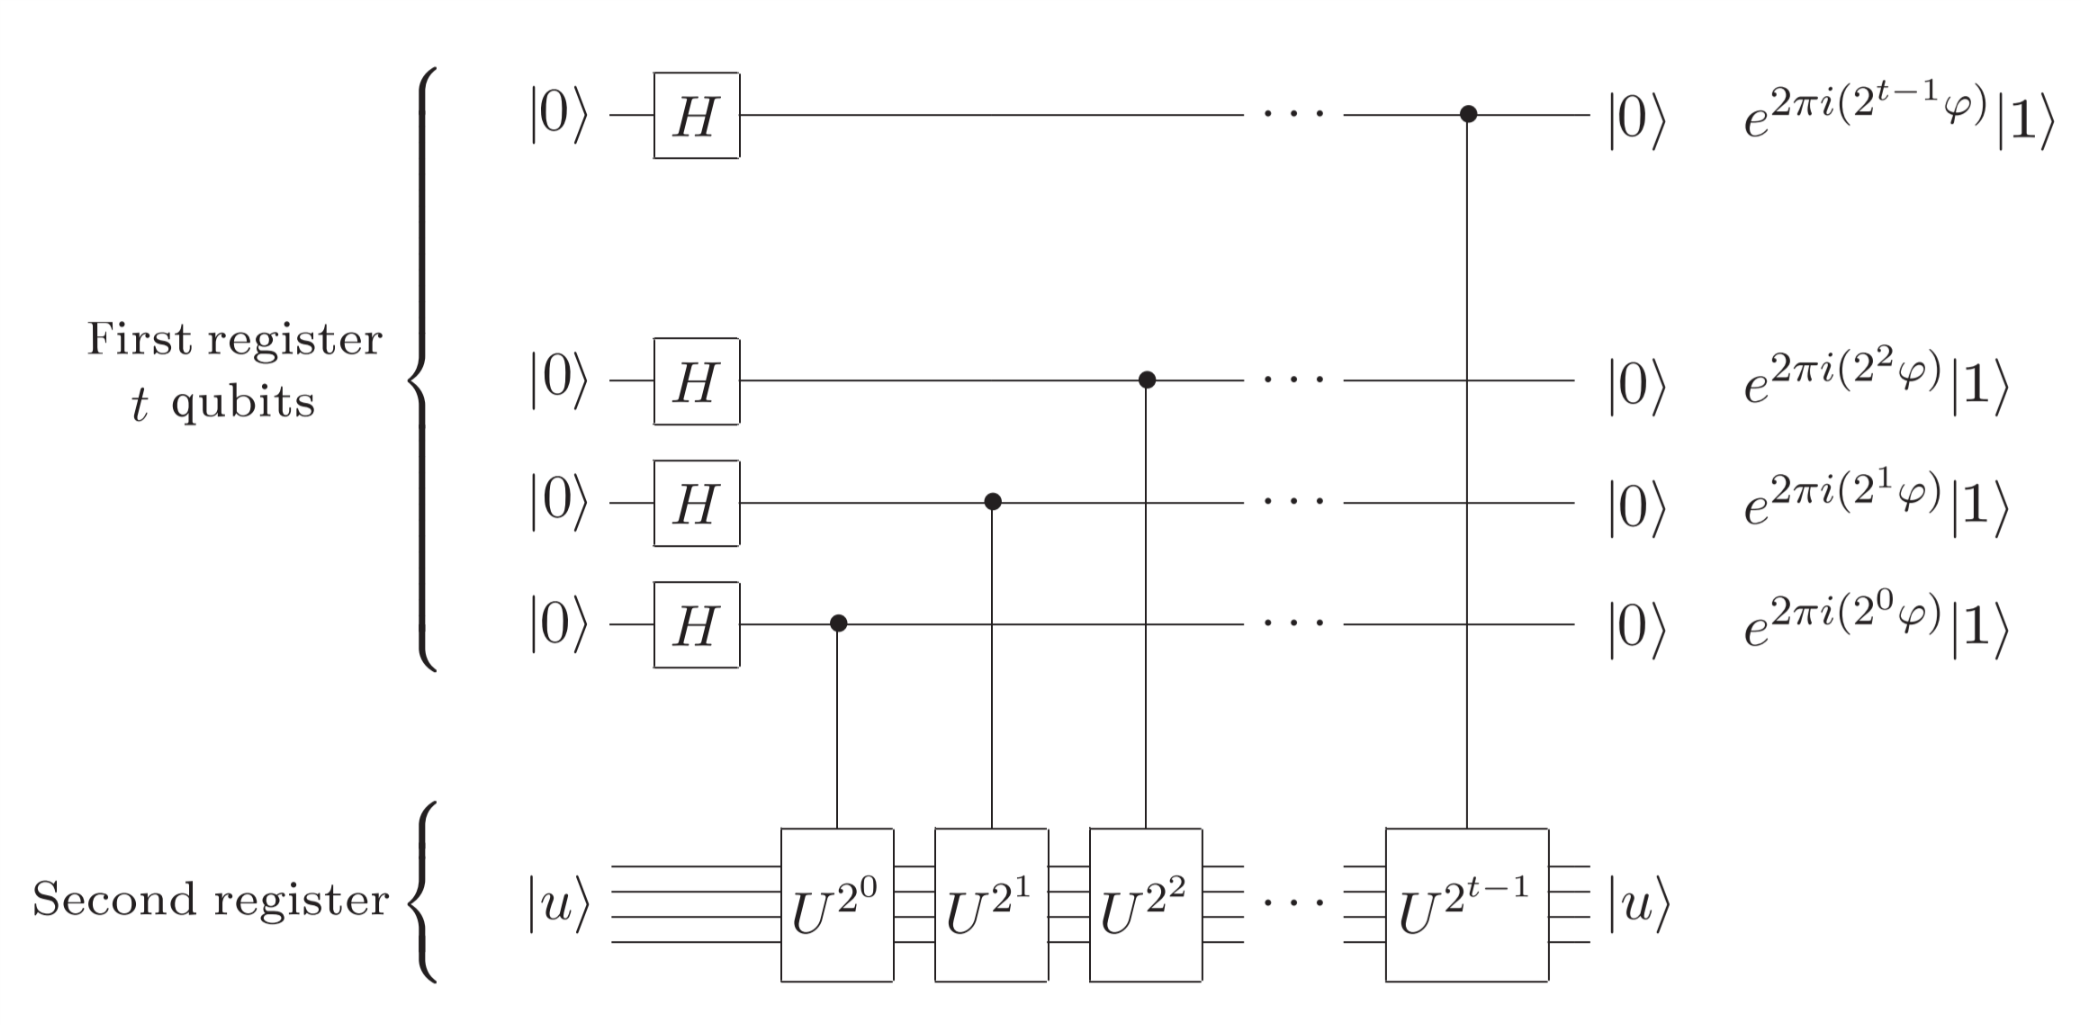
\includegraphics{./others/pe2.png} \emph{Figure 1: The first stage of
  the phase estimation procedure}
\item
  Apply inverse Fourier transform circuit on first register while doing
  nothing on second one. The Fourier transform circuit is shown in
  Figure 2 and the normalization factors and swap gates which should be
  applied at the circuit are not shown. The circuit begins by applying a
  Hadamard transform , followed by application of controlled-\(R_i\)
  operations where operation \(R_k\)'s matrix representation is
  \(\begin{pmatrix}1 & 0 \\0 & e^{2 \pi i / 2^k}\end{pmatrix}\). Finally
  it ends with a swap gate to swap \(\left|{\phi_i}\right\rangle\) and
  \(\left|{\phi_{n-i+1}}\right\rangle\).
  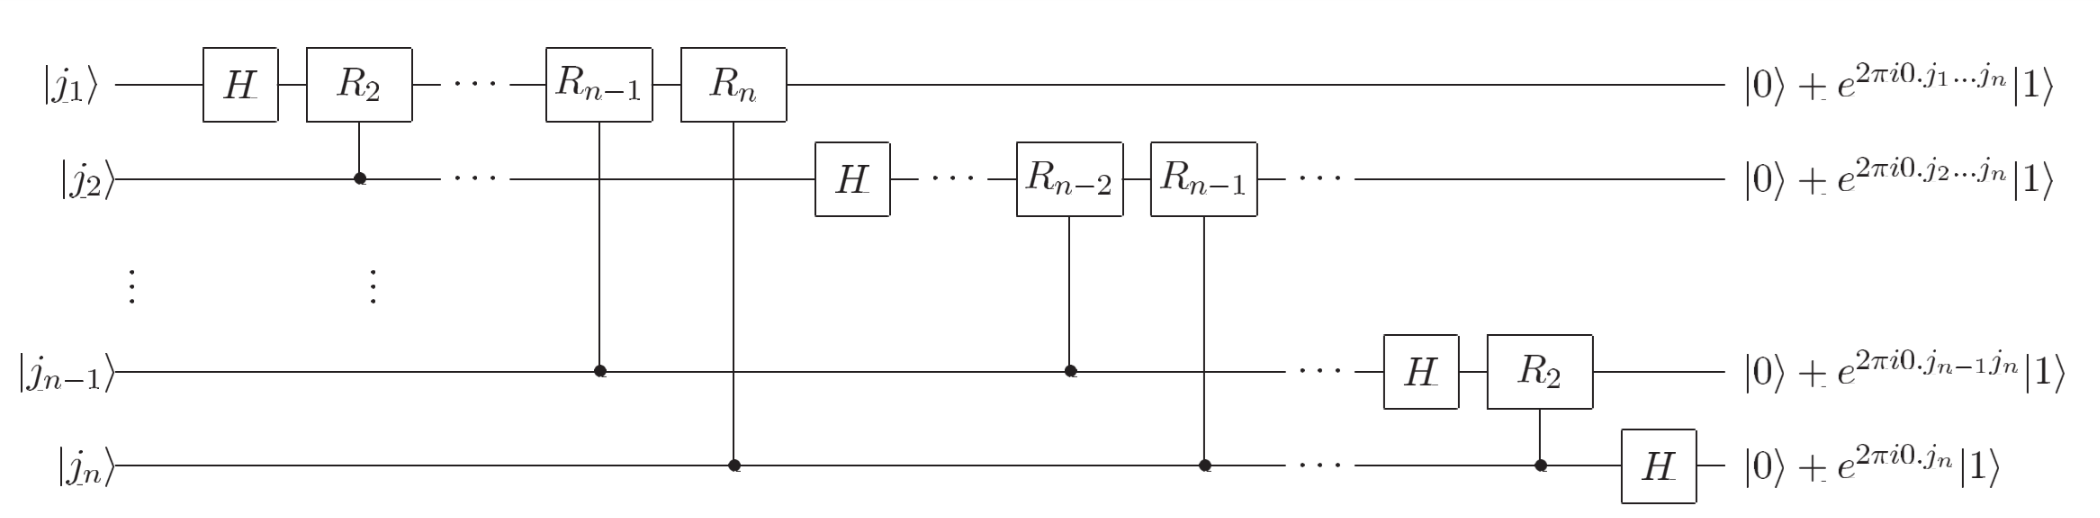
\includegraphics{./others/qft.png} \emph{Figure 2: Quantum Fourier
  Transform circuit}
\item
  The final state of first register is \(\left|{\theta}\right\rangle\)
  where \(\theta\) is a t bit estimation of a element in \$\{\frac{s}{r}
  \textbar{} \(r is the order\), s=0 \dots r-1\}\$. Measure the first
  register and get a decimal \(\theta\).
\end{enumerate}

\subsection{Cross-language
Interoperability}\label{cross-language-interoperability}

To encapsulate the quantum subroutine implemented in Q\#, we separate
the Q\# operations as a standalone .NET standard library project. And we
compiled this project to generate the library assemblies. Then one can
use operations in that library in languages other than C\# by adding a
reference to the assemblies file. For instance, to use our Q\# library
in Python, one could use the Python.NET package to load the assemblies,
and one should also add references to the assemblies from the Q\#
development kit released by Microsoft as dependencies.

The following example shows how to load our assemblies in Python. One
should first have Python.NET package installed in Python environment in
order to use the clr module. One can use the command
\texttt{pip\ install\ pythonnet} to install Python.NET package. It is
also needed to add the path to the assemblies file in the system path
such that the \texttt{clr} module could find the assemblies. Another
requirement is Python library \texttt{qsharp}, which provides a
QuantumSimulator class which wraps the
Microsoft.Quantum.Simulation.Simulators.QuantumSimulator .NET class
provided with the Quantum Development Kit. This wrapper provides a few
useful convienence features that we will use later.

    \begin{Verbatim}[commandchars=\\\{\}]
{\color{incolor}In [{\color{incolor} }]:} \PY{k+kn}{import} \PY{n+nn}{sys}
        \PY{n}{sys}\PY{o}{.}\PY{n}{path}\PY{o}{.}\PY{n}{append}\PY{p}{(}\PY{l+s+s1}{\PYZsq{}}\PY{l+s+s1}{./myShorLib/bin/Release/netstandard2.0}\PY{l+s+s1}{\PYZsq{}}\PY{p}{)}
\end{Verbatim}


    \begin{Verbatim}[commandchars=\\\{\}]
{\color{incolor}In [{\color{incolor} }]:} \PY{k+kn}{import} \PY{n+nn}{qsharp}
\end{Verbatim}


    \begin{Verbatim}[commandchars=\\\{\}]
{\color{incolor}In [{\color{incolor} }]:} \PY{k+kn}{import} \PY{n+nn}{clr}
        \PY{n}{clr}\PY{o}{.}\PY{n}{AddReference}\PY{p}{(}\PY{l+s+s2}{\PYZdq{}}\PY{l+s+s2}{Microsoft.Quantum.Canon}\PY{l+s+s2}{\PYZdq{}}\PY{p}{)}
        \PY{n}{clr}\PY{o}{.}\PY{n}{AddReference}\PY{p}{(}\PY{l+s+s1}{\PYZsq{}}\PY{l+s+s1}{myShorLib}\PY{l+s+s1}{\PYZsq{}}\PY{p}{)}
\end{Verbatim}


    Here \texttt{myShorLib} is the quantum library we implemented in Q\#.
Having added reference to the assemblies, we can now use operations in
the library. To call the operation, we could just import it just as a
normal Python package.

    \subsection{Parallel computation}\label{parallel-computation}

In Shor's algorithm, we use the quantum phase estimation subroutine to
find the order \(r\) of a random number \(x < N\), i.e. a positive
number \(r\) such that \[x^r \equiv 1 \pmod N\] We introduced parallel
computation in this process, that is, performing the order finding
subroutine for multiple random numbers simultaneously with
multi-threading technique. This could accelerate the process of Shor's
algorithm when \(N\) is large. With the help of the cross-language
interoperability of our implementation of the phase estimation
subroutine, we can easily implement the parallel part in Python.

    \begin{Verbatim}[commandchars=\\\{\}]
{\color{incolor}In [{\color{incolor} }]:} \PY{n}{threadPool} \PY{o}{=} \PY{n}{ThreadPool}\PY{p}{(}\PY{n}{processes}\PY{o}{=}\PY{n+nb+bp}{self}\PY{o}{.}\PY{n}{Thread\PYZus{}Num}\PY{p}{)}
        \PY{n}{results} \PY{o}{=} \PY{p}{[}\PY{p}{]}
        \PY{k}{for} \PY{n}{x} \PY{o+ow}{in} \PY{n}{xlist}\PY{p}{:}
            \PY{n}{results}\PY{o}{.}\PY{n}{append}\PY{p}{(}\PY{n}{threadPool}\PY{o}{.}\PY{n}{apply\PYZus{}async}\PY{p}{(}
                \PY{n+nb+bp}{self}\PY{o}{.}\PY{n}{order\PYZus{}finding}\PY{p}{,} \PY{n}{args}\PY{o}{=}\PY{p}{(}\PY{n}{x}\PY{p}{,} \PY{n}{n}\PY{p}{)}\PY{p}{)}\PY{p}{)}
        \PY{n}{threadPool}\PY{o}{.}\PY{n}{close}\PY{p}{(}\PY{p}{)}
        \PY{n}{threadPool}\PY{o}{.}\PY{n}{join}\PY{p}{(}\PY{p}{)}
        \PY{n}{results} \PY{o}{=} \PY{p}{[}\PY{n}{r}\PY{o}{.}\PY{n}{get}\PY{p}{(}\PY{p}{)} \PY{k}{for} \PY{n}{r} \PY{o+ow}{in} \PY{n}{results}\PY{p}{]}
\end{Verbatim}


    For example, when we calls the code to factorize 21. The code will
calculate several \(x\) at the same time, and get the result in a short
time. The process is shown in the figure below.
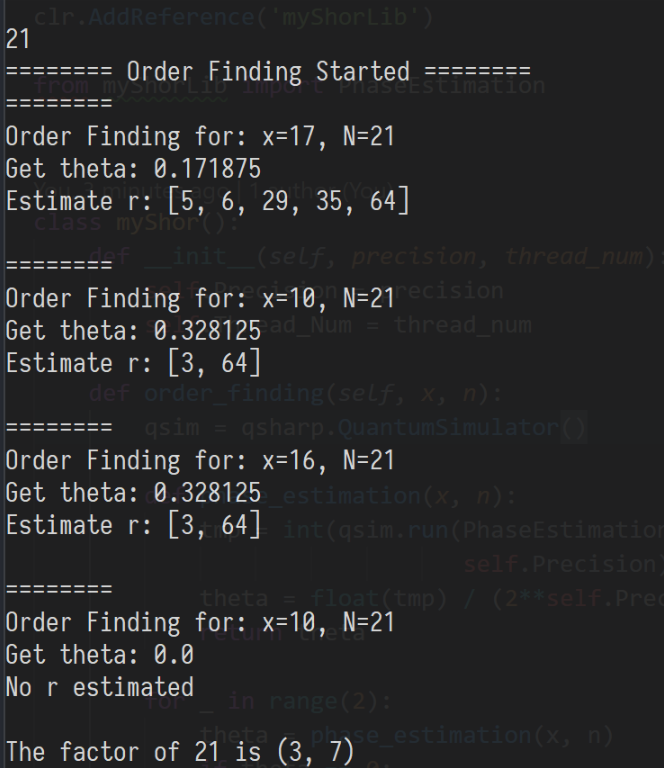
\includegraphics{./others/parallel.png}


    % Add a bibliography block to the postdoc
    
    
    
    \end{document}
